\section{Materials and Methods}
\label{sec:methods}

Each design choice answers a gap of Section~\ref{subsec:gaps}: a multi-object detector instead of a classifier (G1), a swarm optimizer applied to a detector's training hyperparameters (G2), an equal-budget comparison with random search and the defaults, judged with confidence intervals on a test split used once (G3), and separate studio, real-world and Indian test sets (G4).

\subsection{Experimental Design}
\label{subsec:design}

Three arms choose the training hyperparameters of one detector (Fig.~\ref{fig:pipeline}). \armA uses the Ultralytics defaults without search and is the reference any tuning must beat; \armB takes the best of 32 random samples, and \armC the best setting found by a particle swarm of 8 particles over 4 rounds. Both search arms score candidates with the same proxy training (Section~\ref{subsec:proxy}), so the budget is counted in proxy trainings, not in wall-clock time, which varied between methods and cloud sessions (Section~\ref{subsec:res-cost}). Each arm's chosen setting is trained once with an identical recipe (Section~\ref{subsec:training}) and scored once on a held-out test split (Section~\ref{subsec:eval}).

The experiment was run twice. \genone uses one studio-style dataset with six classes at 416~px; \gentwo adds real-world training photographs, a seventh class (OTHER), 640~px images and a test-only Indian set. Search space, PSO settings, seeds, recipes and evaluation code are shared, and both searches were rerun from scratch. Since classes, image size and training data differ, the two generations' scores are not one benchmark; their dedicated comparison is described in Section~\ref{subsec:eval}.

\begin{figure}[!t]
\centering
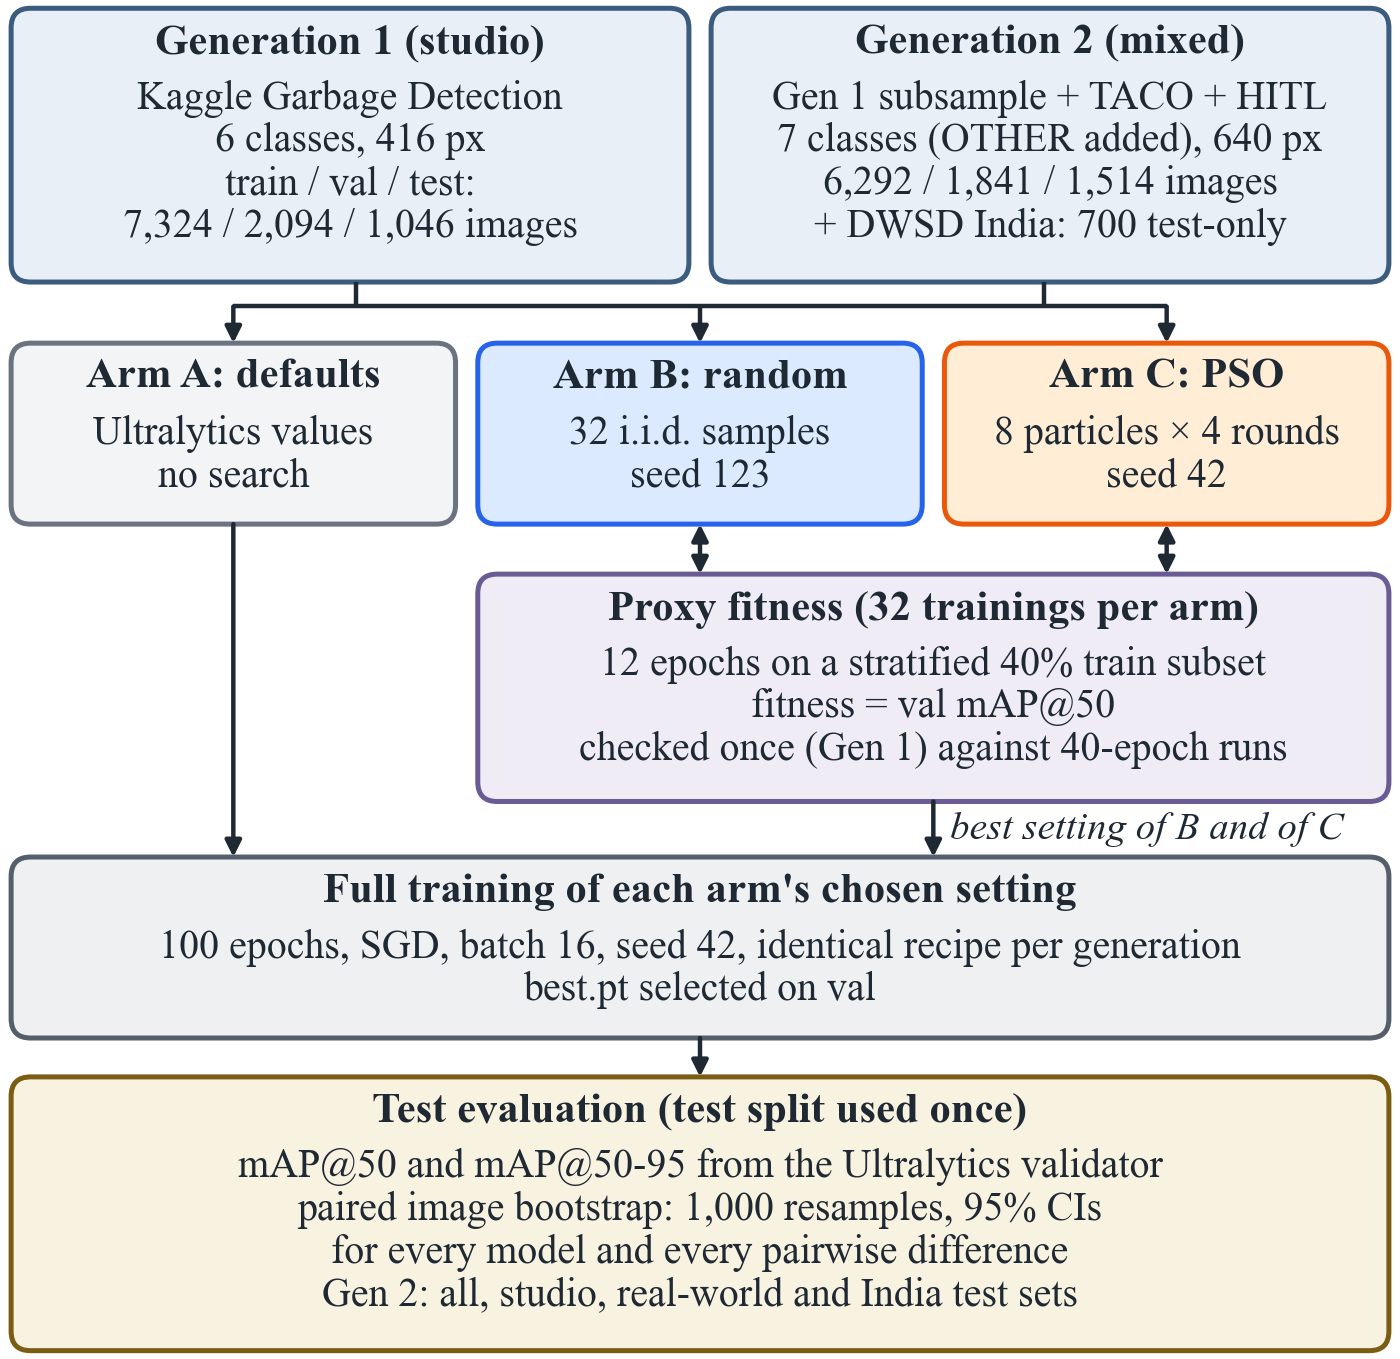
\includegraphics[width=\columnwidth]{m_pipeline.png}
\caption{Experimental pipeline shared by both generations. Arms~B and~C each spend 32 proxy trainings; Arm~A uses the library defaults without search. Each arm's chosen setting is trained once for 100 epochs and tested once.}
\label{fig:pipeline}
\end{figure}

\subsection{Datasets}
\label{subsec:datasets}

Table~\ref{tab:datasets} lists every source with its licence and split sizes.

\textit{\genone data.} The Kaggle dataset ``Garbage Detection -- 6 Waste Categories''~\cite{viswaprakash2024garbage}, from a Roboflow project, holds studio-style images with YOLO boxes in six classes: BIODEGRADABLE, CARDBOARD, GLASS, METAL, PAPER and PLASTIC. In training, 36.45\% of the boxes cover less than 1\% of the image, and BIODEGRADABLE holds 61.92\% of the boxes against 5.61\% for PAPER. The provided folders are split by class (the validation folder has 13,632 BIODEGRADABLE but 33 PAPER boxes, the test folder no GLASS box), so we pooled all images and re-split them 70/20/10, stratified by source class (seed 42), with at least 30 boxes per class in validation and test. Near-duplicates stay in one split: images count as copies if their files are identical (MD5), share a Roboflow source image, or have 256-bit difference hashes within 10 bits, or within 40 bits with a Pearson correlation of at least 0.90 between $64\times64$ grayscale thumbnails. This found 47 groups (133 images). The label checks found 17 zero-size boxes and no corrupt or unlabeled image.

\textit{\gentwo training data.} \gentwo has seven classes: the six \genone classes, with unchanged indices, plus OTHER. A subsample of the \genone splits, stratified by dominant class (seed 42), keeps 3,000 training and 900 validation images, and all test images are kept, so the \gentwo studio test set is the \genone test set. TACO~\cite{proenca2020taco} adds crowd-sourced photographs of litter in the wild; all 60 categories were mapped (for example, drink cans to METAL, cigarettes to OTHER), giving 1,260 OTHER but only 8 BIODEGRADABLE boxes. The HITL Recycling dataset~\cite{hitl2026recycling} adds street photographs, almost all with one litter box, classed by the object tag where decisive (food waste $\to$ BIODEGRADABLE), otherwise by the material tag (aluminum $\to$ METAL), else OTHER; 100 objects lacked a material tag. TACO and HITL were split 70/20/10 with the same duplicate rules and stored with a long side of at most 640~px. The merged data have 962 duplicate groups, none spanning two sources or splits; 918 byte-identical pairs inside the real-world sources cause no leakage but give some photographs extra weight. BIODEGRADABLE holds 51.96\% of the training boxes and OTHER 3.89\%; the studio images have no OTHER box, and the real-world test set a single BIODEGRADABLE box.

\textit{Indian test set.} The Dense Waste Segmentation Dataset (DWSD)~\cite{ali2025dwsd} has 784 phone photographs of streets, parks and garbage areas in Kolkata and Berhampore, West Bengal, annotated as $448\times448$ semantic masks. We used it only for testing, never for training, search or model selection. Each 8-connected region of one mask value (of at least 50 pixels) became a box, so touching items of one class merge into one large box. The class mapping had to be inferred: the published table of mask values does not match what the regions show (the value listed as background covers polythene bags in 610 masks), so we named each value by inspecting its regions; six of the fifteen remain uncertain. The 84 images without boxes were excluded, as some show unannotated waste, leaving 3,040 PLASTIC, 1,230 PAPER, 124 CARDBOARD, 90 OTHER and 18 METAL boxes. An MD5 cross-check against the 9,647 main-build images found no identical file.

\begin{table*}[!t]
\centering
\caption{Datasets. Counts are images, with boxes in parentheses. ``Classes'' is the number of target classes that occur in the source. The \gentwo studio test set equals the \genone test set; the \gentwo real-world test set is the union of the TACO and HITL test images (468 images, 779 boxes).}
\label{tab:datasets}
\footnotesize
\setlength{\tabcolsep}{4pt}
\begin{tabular}{@{}llllllccc@{}}
\toprule
Generation & Source & Domain & Licence & Stored size & Classes & Train & Validation & Test \\
\midrule
\genone & Garbage Detection (Kaggle) & studio & CC BY 4.0 & $416\times416$ & 6 & 7,324 (51,756) & 2,094 (14,904) & 1,046 (7,413) \\
\midrule
\multirow{5}{*}{\gentwo} & \genone subsample & studio & CC BY 4.0 & $416\times416$ & 6 & 3,000 (22,206) & 900 (6,904) & 1,046 (7,413) \\
 & TACO~\cite{proenca2020taco} & real-world & CC BY 4.0 & long side $\le 640$ & 7 & 1,050 (3,293) & 301 (1,031) & 149 (460) \\
 & HITL Recycling & real-world & CC0 & long side $\le 640$ & 7 & 2,242 (2,246) & 640 (641) & 319 (319) \\
 & Total (7 classes) & mixed & & & 7 & 6,292 (27,745) & 1,841 (8,576) & 1,514 (8,192) \\
 & DWSD~\cite{ali2025dwsd} & India & CC BY 4.0 & $448\times448$ & 5 & -- & -- & 700 (4,502) \\
\bottomrule
\end{tabular}
\end{table*}

\subsection{Detector}
\label{subsec:detector}

All arms train YOLOv8n, the nano variant of the YOLOv8 single-stage detectors~\cite{redmon2016you,jocher2023ultralytics}, with Ultralytics 8.4.169, starting from COCO-pretrained weights~\cite{lin2014microsoft} with the class outputs resized to our six or seven classes. The nano model suits a smart bin or phone with limited compute and keeps 32 proxy trainings per arm affordable on one cloud GPU.

\subsection{Search Space}
\label{subsec:space}

Both search arms explore the same six dimensions (Table~\ref{tab:space}): the initial learning rate \texttt{lr0}, the final learning rate as a fraction of it (\texttt{lrf}), the SGD \texttt{momentum}, the \texttt{weight\_decay}, the probability of mosaic augmentation (\texttt{mosaic}) and the gain of random rescaling (\texttt{scale}). The optimizers work in ``search units'': \texttt{lr0} and \texttt{weight\_decay}, which span two orders of magnitude, are held as base-10 exponents (a particle at $-3.2$ means $\texttt{lr0}=10^{-3.2}$), the others as values; decoded values are rounded to six significant digits. Three defaults lie on the boundary, \texttt{lrf} on the lower bound and \texttt{lr0} and \texttt{mosaic} on the upper bounds, so the searches reach them only at the edge. All other training hyperparameters kept the library defaults in every arm.

\begin{table}[!t]
\centering
\caption{Search Space and Search Settings (Shared by Both Generations)}
\label{tab:space}
\footnotesize
\begin{tabular}{@{}p{0.27\columnwidth}lll@{}}
\toprule
Hyperparameter & Range & Scale & Default (Arm~A) \\
\midrule
\texttt{lr0} & $10^{-4}$ to $10^{-2}$ & $\log_{10}$ & 0.01 \\
\texttt{lrf} & 0.01 to 0.2 & linear & 0.01 \\
\texttt{momentum} & 0.60 to 0.98 & linear & 0.937 \\
\texttt{weight\_decay} & $10^{-5}$ to $10^{-3}$ & $\log_{10}$ & 0.0005 \\
\texttt{mosaic} & 0.0 to 1.0 & linear & 1.0 \\
\texttt{scale} & 0.2 to 0.8 & linear & 0.5 \\
\midrule
Setting & \multicolumn{3}{l@{}}{Value} \\
\midrule
PSO budget & \multicolumn{3}{p{0.63\columnwidth}@{}}{8 particles $\times$ 4 rounds $=$ 32 evaluations} \\
Inertia $w_t$ & \multicolumn{3}{p{0.63\columnwidth}@{}}{0.9, 0.65, 0.4 (linear over 3 update steps)} \\
$c_1$, $c_2$ & \multicolumn{3}{p{0.63\columnwidth}@{}}{1.5, 1.5} \\
$\mathbf{r}_1$, $\mathbf{r}_2$ & \multicolumn{3}{p{0.63\columnwidth}@{}}{$U(0,1)$, fresh per particle and dimension} \\
Velocity limit & \multicolumn{3}{p{0.63\columnwidth}@{}}{$\pm20\%$ of each range} \\
Initialization & \multicolumn{3}{p{0.63\columnwidth}@{}}{positions uniform in bounds; velocities uniform in $\pm10\%$ of each range} \\
Boundaries & \multicolumn{3}{p{0.63\columnwidth}@{}}{position clipped; velocity of a clipped dimension set to 0} \\
PSO seed & \multicolumn{3}{p{0.63\columnwidth}@{}}{42} \\
Random search & \multicolumn{3}{p{0.63\columnwidth}@{}}{32 i.i.d.\ uniform samples in search units; seed 123} \\
Fitness & \multicolumn{3}{p{0.63\columnwidth}@{}}{validation \mapfifty after a 12-epoch proxy training on a stratified 40\% training subset} \\
\bottomrule
\end{tabular}
\end{table}

\subsection{Particle Swarm Optimization}
\label{subsec:pso}

Arm~C uses a global-best particle swarm optimizer~\cite{kennedy1995particle} with an inertia weight~\cite{shi1998modified}, hand-written in NumPy, that maximizes the proxy fitness. Particle $i$ has a position $\mathbf{x}_i \in \mathbb{R}^6$ in search units, a velocity $\mathbf{v}_i$ and its best visited position $\mathbf{p}_i$; $\mathbf{g}$ is the swarm's best. One update step is
\begin{equation}
\mathbf{v}_i \leftarrow w_t\,\mathbf{v}_i + c_1\,\mathbf{r}_1 \odot (\mathbf{p}_i - \mathbf{x}_i) + c_2\,\mathbf{r}_2 \odot (\mathbf{g} - \mathbf{x}_i),
\label{eq:velocity}
\end{equation}
where $\odot$ is the element-wise product and $\mathbf{r}_1$, $\mathbf{r}_2$ are redrawn at every step (Table~\ref{tab:space}). Each component $v_{i,d}$ is then clamped to $[-v_{\max,d},\, v_{\max,d}]$ with $v_{\max,d} = 0.2\,(u_d - l_d)$, where $l_d$ and $u_d$ are the bounds of dimension $d$, and
\begin{equation}
\mathbf{x}_i \leftarrow \min\bigl(\max(\mathbf{x}_i + \mathbf{v}_i,\ \mathbf{l}),\ \mathbf{u}\bigr),
\label{eq:position}
\end{equation}
element-wise; a clipped dimension's velocity is set to zero, so the particle rests at the wall. Round~1 evaluates the random initial swarm, and each of the $T-1 = 3$ update steps is followed by one more round, so $T = 4$ rounds use exactly 32 evaluations. The inertia weight falls linearly,
\begin{equation}
w_t = w_{\mathrm{start}} - (w_{\mathrm{start}} - w_{\mathrm{end}})\,\frac{t-1}{T-2}, \qquad t = 1, \dots, T-1,
\label{eq:inertia}
\end{equation}
from $w_{\mathrm{start}} = 0.9$ to $w_{\mathrm{end}} = 0.4$. The inertia weight is the concept of~\cite{shi1998modified}; this linear schedule is our setting, chosen so that the swarm explores first and refines later. A personal best is replaced only by a strictly higher fitness. All randomness comes from one seeded generator, so an interrupted search resumes exactly by replaying the seed and the logged fitness values. A failed training (non-finite \mapfifty) would get fitness 0 and never be selected; none occurred in the four searches.

As a code check, with 20 particles, 50 rounds and 10 seeds on $[-5.12, 5.12]^6$, the median best value was $1.9\times10^{-5}$ on Sphere and 6.96 on the multimodal Rastrigin function (both with minimum 0): the optimizer converges on a smooth bowl and keeps improving among many local minima. This makes no claim about tuning performance.

\subsection{Random Search and Defaults}
\label{subsec:random}

Arm~B draws 32 points uniformly in search units (log-uniform for \texttt{lr0} and \texttt{weight\_decay}) and scores them with the same proxy and script as the swarm. Random search~\cite{bergstra2012random} is included because any structured optimizer should beat it at the same budget. Each search arm's winner is its highest proxy fitness (the first on a tie). Arm~A uses the defaults in Table~\ref{tab:space}.

\subsection{Proxy Fitness and Its Validation}
\label{subsec:proxy}

A full training takes over an hour on our GPU, so the searches score candidates with a 12-epoch proxy training on a stratified 40\% training subset: 2,930 of the 7,324 \genone images (by source class) and 40\% of the 6,292 \gentwo images (by source and dominant class). The subset is drawn once (seed 42) and stored as an image list, so every candidate trains on the same images. The fitness is the validation \mapfifty of the last-epoch weights. The proxy follows the full-training recipe (Section~\ref{subsec:training}), except that the no-mosaic period and the warm-up keep their share of the run, 10\% and 3\% (\texttt{close\_mosaic} 1 epoch, warm-up 0.36 epochs), which keeps the searched \texttt{mosaic} faithful to the full run.

Before the \genone searches, we tested whether the proxy ranks settings like a longer training. Seven configurations drawn by Latin hypercube sampling~\cite{mckay1979comparison} in search units (SciPy, ``random-cd'', seed 42) plus the defaults were each trained with the proxy and with a 40-epoch ``medium'' run on the full training split (\texttt{close\_mosaic} 4, warm-up 1.2 epochs), both at 416~px. The statistic was the Spearman rank correlation~\cite{spearman1904proof} of the eight score pairs; the pass threshold, $\rho \ge 0.6$, and the fallback, a 20-epoch proxy, were fixed in advance (results in Section~\ref{subsec:res-proxy}).

The check was not repeated for \gentwo; the decision, recorded before its searches, relied on the \genone result and the unchanged recipe, so proxy validity under the new data, classes and image size is assumed, not tested. The check also has only eight configurations and a 40-epoch rather than 100-epoch reference, and the proxy scores last-epoch weights while the final models use \texttt{best.pt} (Section~\ref{subsec:limitations}).

\subsection{Full Training}
\label{subsec:training}

Each arm's chosen setting was trained once from the COCO-pretrained weights for 100 epochs on the full training split, with an identical recipe for the three arms: SGD set explicitly (the default \texttt{optimizer=auto} would ignore the searched \texttt{lr0} and \texttt{momentum}; each run records the optimizer and learning rate used), batch size 16, a 3-epoch warm-up, no mosaic in the last 10 epochs, and 416~px in \genone or 640~px in \gentwo. The checkpoint with the best validation fitness (\texttt{best.pt}) was tested; other arguments kept their defaults.

Every run used seed 42 in deterministic mode. A module that Ultralytics imports lazily during a process's first training draws random numbers after seeding, so first runs differed from later ones; importing it before seeding removed the difference. All trainings ran on one NVIDIA Tesla T4 GPU on Kaggle, with one training seed per arm, so run-to-run variance is not measured (Section~\ref{subsec:limitations}).

Two \gentwo runs froze, most likely because the session's data mount stopped responding. Arm~C was resumed from its epoch-55 checkpoint after checking every saved training argument against the plan; this continues the same weights, optimizer state and epoch counter but is not bit-identical to an uninterrupted run. The random search, stopped after 11 of 32 evaluations, was continued by replaying its log, which affected no completed evaluation.

\subsection{Evaluation Protocol}
\label{subsec:eval}

Each test split was scored once, after all training; trial evaluations used the validation split. In \gentwo, one run scored the three models on the whole test split (``all'', 1,514 images) and separately on the studio, real-world and India sets. Each checkpoint first had to match its arm's record (classes, epochs, image size, the six hyperparameters).

The Ultralytics validator ran at each model's training image size (batch 32, rectangular batching, confidence threshold 0.001, NMS IoU 0.7, 32-bit floats). We report \mapfifty, \mapfiftyninetyfive (IoU 0.50 to 0.95 in steps of 0.05), precision and recall at the maximum-F1 confidence, and per-class AP@50. Both mAP values, recomputed from the stored per-image statistics, had to match the validator within $10^{-4}$; they agreed exactly everywhere.

Uncertainty comes from a paired image bootstrap~\cite{efron1993introduction}: 1,000 resamples of the test images (seed 0), with the same indices for every model. We report 95\% percentile intervals for each model and each pairwise difference; a difference is significant only if its interval excludes 0. Each \gentwo test set has its own bootstrap. No $p$-values or multiple-comparison corrections were computed, per-class AP has no interval, and the intervals cover test sampling only, not training or search randomness.

To compare the generations on the same images, all six final models (three arms per generation) were scored on the studio and real-world test sets, each at its own training image size, with labels restricted to the six shared classes: OTHER labels were removed (images left empty stay in), and \gentwo's OTHER predictions were dropped in non-maximum suppression. Each test set has its own bootstrap. The results are in Section~\ref{subsec:res-domain} and Table~\ref{tab:g1g2}.

Inference speed is the median batch-1 latency over 100 test images after 10 warm-up predictions (confidence 0.25) at the training image size, on a laptop CPU (Intel Core Ultra~5 125H) for \genone and on the T4 GPU for \gentwo, so it is comparable only within a generation.
